\subsection{Kommandozeilenprogramm Design-SVG-Konverter}
Nach der, in Kapitel \ref{Kommandozeilenprogramm Adobe-Illustrator-Designkonvertierung} \emph{Kommandozeilenprogramm Adobe-Illustrator-Designkonvertierung} beschrieben, Konvertierung der Designvorlagen, werden Derivate der Vorlagen erzeugt. Diese enthalten übersetzte Texte, für die unterschiedlichen Sprachen in denen die Vorlagen angeboten werden. Um die Vielfalt der Vorlagen zu erhöhen, werden außerdem weitere Derivate mit unterschiedlichen Farbzuordnung erzeugt. Die Erzeugung der Derivate ist nicht Bestandteil des FreeDesign-Projektes. Jedoch werden in einem letzten Prozessschritt 3D-Vorschaubilder der Derivate zur Präsentation im Webshop erzeugt. Die Erzeugung der Vorschaubilder, die ebenfalls nicht Teil des FreeDesign-Projektes ist, basiert auf SVG-Dateien die durch das FreeDesign-Projektes erzeugt werden. Hier zu 


Konvertierung der Designvorlagen, werden in einem weiteren Prozessschritt 3D-Vorschaubilder für die Präsentation im Webshop erzeugt. 

Das FreeDesign-Projekt unterstützt den, im Kapitel \ref{Kommandozeilenprogramm Adobe-Illustrator-Designkonvertierung} \emph{Kommandozeilenprogramm Adobe-Illustrator-Designkonvertierung} beschrieben, Import der Designvorlagen durch ein weiteres Kommandozeilenprogramm. 

\begin{figure}[H]
    \centering
    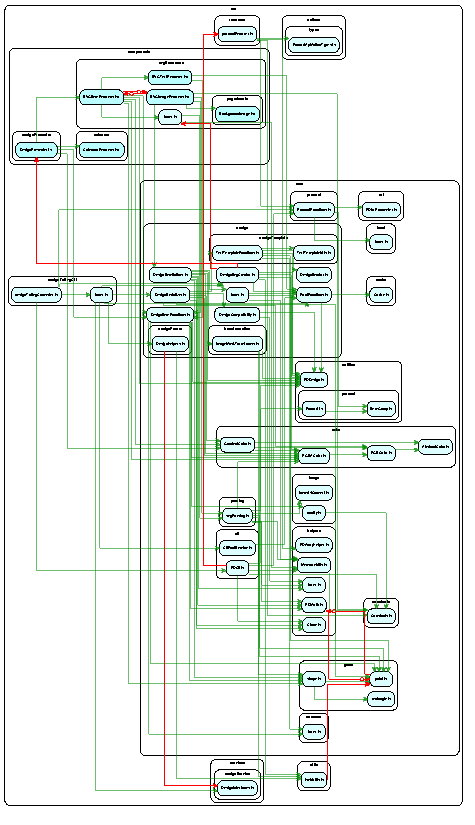
\includegraphics{diagrams/Ist-Architektur/designToSvgCLI-analysis.pdf}
    \caption{Abhängigkeiten der Komponenten für das Kommandozeilenprogramm zur Konvertierung von Designs zu SVG-Dateien.}
    \label{fig:DesignToSvg}
\end{figure}
\begin{multicols}{2}
    \begin{enumerate}
    \item API-Kommunikation
    \item Bildverarbeitung
    \item Cache
    \item Designdarstellung
    \item Design-Parser
    \item Design-Serialisierung
    \item Designstruktur
    \item Farbstruktur
    \item JavaScript-Erweiterung
    \item Mathematik
    \item Maßeinheit-Konverter
    \item Produktstruktur
    \item Schriftverarbeitung
    \item SVG-Parser
    \item Vorlagekonverter
\end{enumerate}

\end{multicols}